\documentclass[border=4pt]{standalone}
\usepackage{tikz}
\usetikzlibrary{arrows.meta,positioning,fit}
\begin{document}
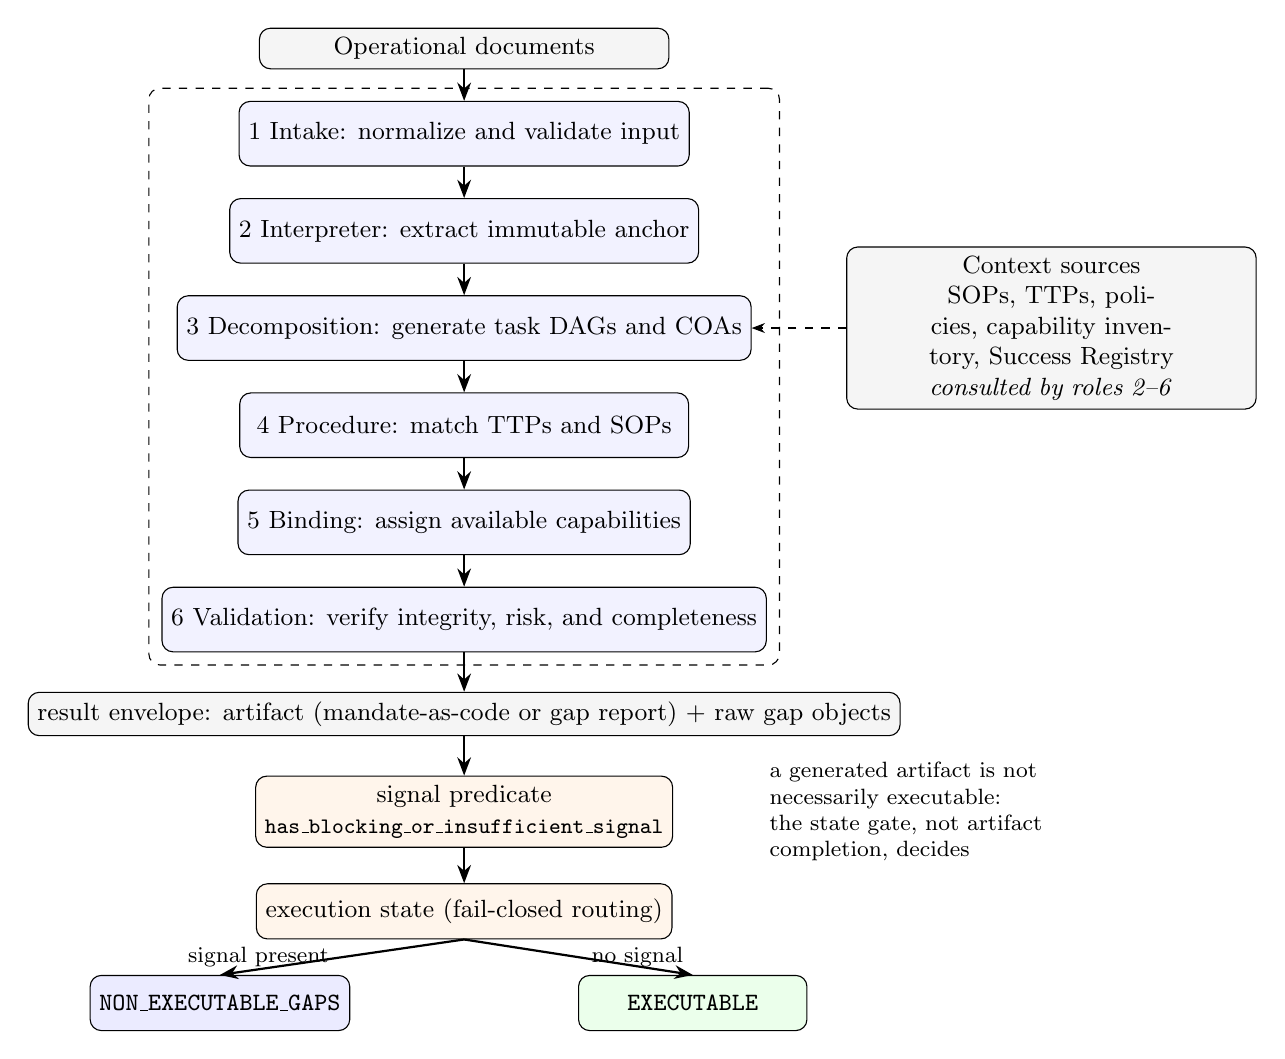
\begin{tikzpicture}[>=Stealth, every node/.style={font=\small},
  role/.style={draw, rounded corners, align=center, minimum width=5.7cm, minimum height=0.82cm, fill=blue!5},
  src/.style={draw, rounded corners, align=center, minimum width=5.2cm, fill=gray!8},
  gate/.style={draw, rounded corners, align=center, minimum width=3.4cm, minimum height=0.7cm, fill=orange!8},
  term/.style={draw, rounded corners, align=center, minimum width=2.9cm, minimum height=0.7cm, font=\small\ttfamily}]
\node[src] (input) {Operational documents};
\node[role, below=0.40cm of input] (intake) {1 Intake: normalize and validate input};
\node[role, below=0.40cm of intake] (interp) {2 Interpreter: extract immutable anchor};
\node[role, below=0.40cm of interp] (decomp) {3 Decomposition: generate task DAGs and COAs};
\node[role, below=0.40cm of decomp] (proc) {4 Procedure: match TTPs and SOPs};
\node[role, below=0.40cm of proc] (bind) {5 Binding: assign available capabilities};
\node[role, below=0.40cm of bind] (valid) {6 Validation: verify integrity, risk, and completeness};
\node[src, below=0.50cm of valid] (out) {result envelope: artifact (mandate-as-code or gap report) + raw gap objects};
\node[gate, below=0.50cm of out] (pred) {signal predicate\\{\footnotesize\texttt{has\_blocking\_or\_insufficient\_signal}}};
\node[gate, below=0.45cm of pred] (state) {execution state (fail-closed routing)};
\node[term, below left=0.45cm and -1.2cm of state, fill=blue!8] (nex) {NON\_EXECUTABLE\_GAPS};
\node[term, below right=0.45cm and -1.2cm of state, fill=green!8] (exe) {EXECUTABLE};
\node[src, right=1.2cm of decomp, text width=4.0cm] (sources) {Context sources\\SOPs, TTPs, policies, capability inventory, Success Registry\\\emph{consulted by roles 2--6}};
\foreach \a/\b in {input/intake,intake/interp,interp/decomp,decomp/proc,proc/bind,bind/valid,valid/out,out/pred,pred/state}{\draw[->, thick] (\a) -- (\b);}
\draw[->, thick] (state.south) -- node[left=1pt, font=\footnotesize]{signal present} (nex.north);
\draw[->, thick] (state.south) -- node[right=1pt, font=\footnotesize]{no signal} (exe.north);
\draw[->, dashed] (sources.west) -- (decomp.east);
\node[draw, dashed, rounded corners, fit=(intake)(interp)(decomp)(proc)(bind)(valid), inner sep=0.16cm] {};
\node[right=1.1cm of pred, text width=4.0cm, font=\footnotesize, align=left]
  {a generated artifact is not\\ necessarily executable:\\ the state gate, not artifact\\ completion, decides};
\end{tikzpicture}
\end{document}
